% BML

\def\bml#1{\texttt{\color{blue} #1}}  % Bml routines stile for algorithm.
\newcommand*\mycommand[1]{\texttt{\emph{#1}}}
\newcommand{\bra}[1]{\langle #1 |}
\newcommand{\ket}[1]{| #1 \rangle}
\newcommand{\braket}[2]{\langle #1 | #2 \rangle}
\newcommand{\spec}[1]{\langle #1 \rangle}
\newcommand{\icomp}{\mathrm{i}}
\newcommand{\tr}{\mathrm{Tr}}
\newcommand{\norm}[1]{\Vert #1 \Vert}
\newcommand{\fer}{\mathrm{f}}
\newcommand{\emin}{\epsilon_{\mathrm{min}}}
\newcommand{\emax}{\epsilon_{\mathrm{max}}}  
% \newcommand{\p}{\textbf{P}^{\bot}}
\newcommand{\p}{\textbf{P}}
\newcommand{\pno}{\textbf{P}}
\newcommand{\HH}{\textbf{H}}  
\newcommand{\ham}{\textbf{H}}
% \newcommand{\ham}{\textbf{H}^{\bot}}  
\newcommand{\X}{\textbf{X}}
\newcommand{\Id}{\textbf{I}}
\newcommand{\B}{\textbf{B}}
\newcommand{\SSS}{\textbf{S}}
\newcommand{\C}{\textbf{C}}
\newcommand{\Z}{\textbf{Z}}


  The basic matrix library package (BML) provides a common application programming interface (API) for linear algebra and matrix functions in C and Fortran for quantum chemistry codes. The BML API is matrix format independent. Currently the dense and ELLPACK-R sparse matrix data types are available, each with different implementations. As an example application, we show how the second order spectral projection (SP2) algorithm used to compute the electronic structure of a molecular system represented with a tight-binding (TB) Hamiltonian can be successfully implemented with the aid of this library. 

The increasing availability of different computational architectures (multicore, many-core, accelerated), data storage formats (sparse .vs. dense) and programming models (distributed, threaded, task-based) renders the implementation, testing and optimization of scientific algorithms more and more ``overwhelming'' \cite{Merali2010}. Quantum chemistry packages suffer from this issue since the operations involved are essentially matrix-matrix operations. This has been the focus of countless improvements both from the computational and pure algorithmic point of view \cite{watkins2010}. 
A large development requires the combined efforts of domain scientists (computational chemist/physicist) and computer scientists. 
%
We introduce a library that is matrix storage format agnostic.
This allows lower-level matrix-oriented algorithm implementation to evolve independently of the higher-order solvers. 
This library is primarily focused on matrix linear algebra.
Sharing a similar philosophy, the Matrix Template Library (MTL) \cite{mtl} serves to provide a general solution of matrix formats and algorithms as a C++ library. In contrast, BML provides matrix formats and algorithms relevant to quantum chemistry.

Quantum chemistry packages have a common bottleneck.  They solve a generalized eigenvalue problem in order to obtain a density matrix to characterize the electronic structure of a particular system. The computational cost of solving this generalized eigenvalue problem usually scales as $\mathcal{O}(N^3)$, where $N$ is the number of atomic orbitals of the system. One promising method for computing the density matrix with $\mathcal{O}(N)$ scaling is the second order spectral projection (SP2) \cite{ANiklasson02}. The SP2 algorithm can be implemented using dense or sparse matrices. This algorithm makes possible the quantum-based molecular dynamics (QMD) simulations of proteins of several thousands of atoms on traditional \cite{Mniszewski2015,Negre2016} and GPU-accelerated architectures \cite{MCawkwell_GPU,MCawkwell_MultGPU}. 

The SP2 algorithm is used to illustrate the power of the BML library. Currently, only dense and sparse ELLPACK-R matrix formats are available but efforts to extend this list are ongoing. Plans include the addition of dense matrix on GPU, sparse ELLPACK-R on GPU, Compressed Sparse Row (CSR) matrices on CPUs and GPUs. The algorithm 
implementations are multi-threaded for efficient execution on multi-core single node shared memory architectures. 
A distributed memory multi-node version is under development.

\subsection{Design goals of the library}
\label{design}

Optimized dense linear algebra libraries currently exist such as Linear Algebra Package (LAPACK) \cite{lapack} and Basic Linear Algebra Subprograms (BLAS) \cite{MDayde95} with realizations in
the Intel Math Kernel Library (MKL) \cite{mkl}, AMD Core Math Library (ACML) \cite{acml}, AMD Compute Libraries (ACL)\cite{acl}, and Nvidia BLAS Library (cuBLAS) \cite{cublas}. Libraries for sparse linear algebra are currently limited and lacking in performance. Examples include MKL \cite{mkl}, ACL \cite{acl}, and Nvidia CUDA sparse Matrix Library (cuSPARSE) \cite{cusparse}. Reduced complexity electronic structure applications rely on sparse linear algebra and require hand-tuned implementations of sparse matrix operations.
%, potentially severely limiting the exploitability of future algorithm or computer hardware developments\cite{Mniszewski2015}.
The basic matrix library addresses this challenge by offering high level abstractions for matrix operations independent of the underlying data structures and algorithms.

The BML architecture is shown in Figure 1.
The core of the library is written in C with a thin Fortran glue layer exposing the API to Fortran 9x applications. The exported matrix data type is a \texttt{void} pointer, enabling the library to choose the data structure appropriate implementation at runtime through a series of nested \texttt{switch} statements. This flexibility also enables support of several \texttt{float} variants, i.e.~currently the library supports dense and ELLPACK-R \cite{ellpack} matrix types and single and double precision real and complex \texttt{float} types. Since C does not support generic programming, we use a series of preprocessor macros to emulate such support, minimizing code duplication.
Algorithm implementations are multi-threaded using the Open Multi-Processing \cite{OpenMP} API and multi-threaded
BLAS libraries (ex. MKL).

The types of matrix algorithms available are shown in Table 1. In most cases, variants are available for all matrix formats.

\begin{table}[htbp]
\caption{BML Routines}
\begin{tabular}{ll}
\hline
\multicolumn{1}{l}{Matrix Algorithm} & \multicolumn{1}{l}{Examples } \\ \hline
Addition & \bml{bml\_add}, \bml{bml\_add\_identity}  \\ \hline
Allocation & \bml{bml\_zero\_matrix}, \\
& \bml{bml\_random\_matrix}, \\
& \bml{bml\_identity\_matrix}  \\ \hline
Copy & \bml{bml\_copy} \\ \hline
Getters & \bml{bml\_get\_row}, \bml{bml\_get\_value} \\ \hline
I\/O & \bml{bml\_read\_matrix}, \\
& \bml{bml\_write\_matrix}, \\
& \bml{bml\_print\_matrix} \\ \hline
Introspection & \bml{bml\_get\_N}, \bml{bml\_get\_precision} \\ \hline
Multiply & \bml{bml\_multiply}, \\
& \bml{bml\_multiply\_x2}, \\
& \bml{bml\_multiply\_AB} \\ \hline
Norm & \bml{bml\_fnorm} \\ \hline
Normalize & \bml{bml\_gershgorin}, \bml{bml\_normalize} \\ \hline
Scale & \bml{bml\_scale} \\ \hline
Setters & \bml{bml\_set\_row}, \bml{bml\_set\_value} \\ \hline
Threshold & \bml{bm|\_threshold} \\ \hline
Trace & \bml{bml\_trace} \\ \hline
Transpose & \bml{bml\_transpose} \\ \hline
\end{tabular}
\label{bmlalgtype}
\end{table}

The code is hosted on github \cite{bml} and integrated with travis-ci and codecov.io for continuous integration and code coverage analysis. Every commit is tested over a set of compiler and compiler options.

\begin{center}
  \begin{figure}
    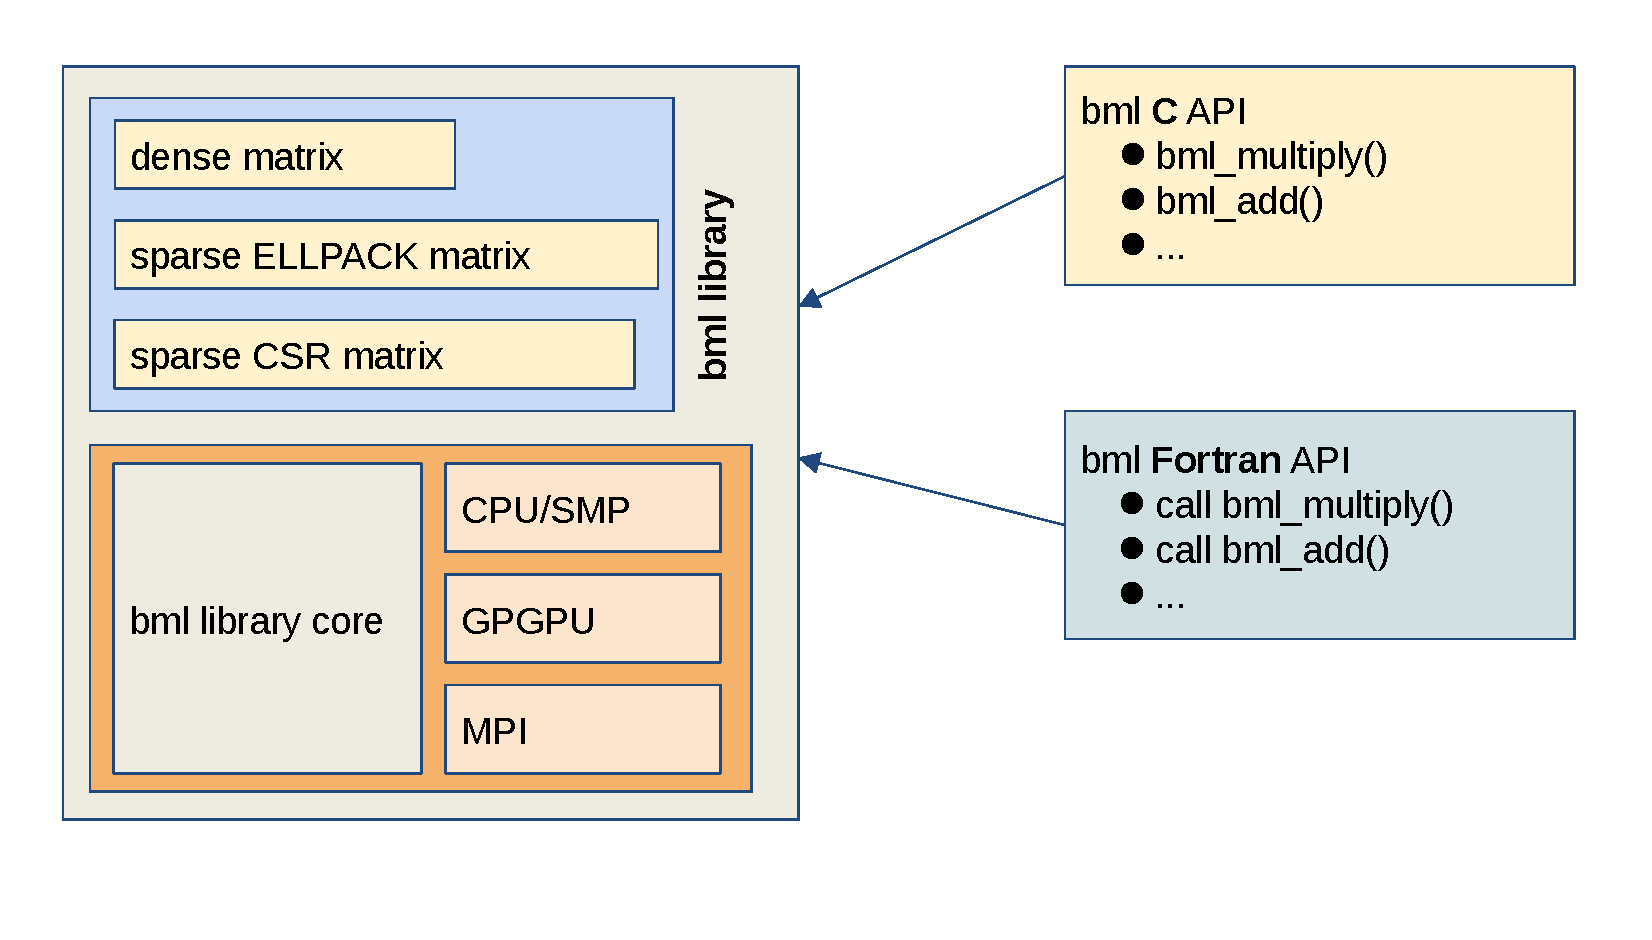
\includegraphics[width=8.0cm]{./fig/bml_scheme.pdf}
    \caption{The Basic Matrix Library (BML) is a set of matrix storage types and algorithms with a common API in C and Fortran. It currently runs on single node multi-core shared memory architectures. Extension to accelerated and distributed memory architectures is under development.
    }
    \label{bmlarch}
  \end{figure} 
\end{center}

The use of this library is very straightforward. In the application code, the BML main module is included. A matrix is declared as follows.  


  \texttt{\textbf{type}(\bml{bml\_matrix\_t}) :: a} 


Next it is allocated given the desired type and precision (e. g. dense and double precision). 
Refer to the manual page on allocation functions for a complete list \cite{bml}. For instance,
%

  \texttt{\textbf{call} \bml{bml\_zero\_matrix}(bml\_matrix\_dense, bml\_precision\_double, 100, a)}

%
will allocate matrix a in dense format, double-precision, 100 x 100 matrix which is initialized to zero. Additional functions allocate
special matrices.
%
\begin{itemize}
  \item \texttt{\textbf{call} \bml{bml\_random\_matrix(...)}} Allocate and initialize a random matrix.
  \item \texttt{\textbf{call} \bml{bml\_identity\_matrix(...)}} Allocate and initialize an identity matrix.
\end{itemize}
%
A matrix is deallocated by calling:
\texttt{\textbf{call} \bml{bml\_deallocate}(a)}

\subsection{Implementation of the SP2 algorithm}

With the density matrix operator $\hat{\rho}$ any expectation value or property $\hat{A}$ can be computed as $\tr(\hat{\rho} \hat{A})$.
%
The density matrix operator can be written as the Fermi function of the Hamiltonian operator $\hat{H}$, this is:   $\hat{\rho} =   \fer(\hat{H})$. When expressed in an orthogonal basis of localized atomic orbitals the latter equation reads:
$\pno_{ij} = \bra{\alpha_i}\hat{\rho}\ket{\alpha_j}= [\C\fer(\bm{\epsilon})\C^\dagger]_{ij}$, where matrices $\bm{\epsilon}$ and $\C$ are the matrices containing the eigenvalues $\epsilon_i$ and eigenvectors $C_{i}$ respectively \cite{Sakurai}. This implies that, in order to construct matrix $\pno$ we need first to solve the eigenvalue problem $\ham \C = \C \epsilon$ which has an $\mathcal{O}(N^3)$ computational cost.

The SP2 method allows us to obtain $\p$ from $\ham$ with linear scaling. It is based on the expansion of the Fermi operator at zero electronic temperature. This is: 

\begin{equation}
  \p =   \Theta[\mu \Id - \ham]
\end{equation}
%
where $\Id$ is the identity matrix. By writing a recursive expansion of $\Theta$, we have: 


\begin{equation}
  \Theta[\mu \Id - \ham] =   \lim_{i \rightarrow \infty} f_i(f_{i-1}(...f_0(\X_0)))
\end{equation}
%
where $\X_0$ is the initial member of the sequence which is computed as: 

\begin{equation}
  \X_0 = \frac{\emax \Id - \ham}{\epsilon_{\mathrm{max}} - \epsilon_{\mathrm{min}}} 
\end{equation}
%
where $\emin$ and $\emax$ are estimated with the Gershgorin circle theorem \cite{GGolub96}. The SP2 uses the sequence of the following projection polynomials: 
%
\begin{equation}
  f_i(\X_i) = \begin{cases} 
    \X_i^2, & \mbox{if } \tr(\X) \leqq N_{occ} \\ 
    2\X_i - \X_i^2, & \mbox{if } \tr(\X) > N_{occ}
  \end{cases}
\end{equation}
%
The recursive function is then applied until $\tr(\X) \simeq N_{occ}$ for when we finally have $\p = \X$.

Pseudocode for this algorithm is given in Algorithm 1, whereas the actual FORTRAN code is given in Algorithms 2 and 3.  

\begin{algorithm}[H]
  \algrenewcommand\algorithmicfunction{\textbf{procedure}}
  \begin{algorithmic}
    \parskip 0.05cm
    {\fontsize{0.3cm}{0.3em}\selectfont 
      \Function{SP2}{tol, $\ham$, $\p$, $N_{\mathrm{occ}}$}
      \State Estimate $\emin$ and $\emax$ from $\ham$
      \State $\X = (\emax \Id - \ham)/(\emax - \emin) $
      \State TraceX = $\tr[\X]$
      \State \textbf{for} $i$ = 1 : $i_{\mathrm{max}}$ \textbf{do}
      \State \qquad TraceXold = TraceX
      \State \qquad $\X_{\mathrm{tmp}}=\X^2$
      \State \qquad \textbf{if} $(\mathrm{TraceX} - N_{\mathrm{occ}}) \leqq 0$ \textbf{then}
      \State \qquad \qquad $\X = 2\X - \X_{\mathrm{tmp}}$
      \State \qquad \textbf{else}
      \State \qquad \qquad $\X = \X_{\mathrm{tmp}}$
      \State \qquad \textbf{end if}
      \State \qquad \textbf{if} $|\mathrm{TraceX} - N_{\mathrm{occ}}| \leqq \mathrm{tol}$ \textbf{then}
      \State \qquad \qquad \textbf{break}
      \State \qquad \textbf{end if}
      \State \textbf{end for}
      \State $\p = \X$
      %     
      \EndFunction
    }       
  \end{algorithmic}
  \label{pcode}
  \caption{Pseudocode for the SP2 algorithm.}
\end{algorithm}

\newcommand{\myvarsf}[1]{\texttt{#1}}
\newcommand{\mynumf}[1]{\textit{#1}}
\newcommand{\eminb}[0]{\myvarsf{emin}}
\newcommand{\emaxb}[0]{\myvarsf{emax}}
\newcommand{\norb}[0]{\myvarsf{Norb}}
\newcommand{\noc}[0]{\myvarsf{Nocc}}
\newcommand{\hbml}[0]{\myvarsf{h\_bml}} 
\newcommand{\pbml}[0]{\myvarsf{rho\_bml}}
\newcommand{\type}[0]{\myvarsf{bml\_type}}
\newcommand{\lprec}[0]{\myvarsf{dp}}
\newcommand{\gb}[0]{\myvarsf{Gersh}}
\newcommand{\elem}[0]{\myvarsf{bml\_element\_real}}
\newcommand{\xx}[0]{\myvarsf{x2\_bml}}
\newcommand{\gf}[0]{\myvarsf{GershFact}}
\newcommand{\thr}[0]{\myvarsf{numthresh}}
\newcommand{\cvar}[0]{\myvarsf{Control\_vars}}
\newcommand{\trxb}[0]{\myvarsf{trx}}
\newcommand{\iter}[0]{\myvarsf{iter}}
\newcommand{\imax}[0]{\myvarsf{imax}}
\newcommand{\tol}[0]{\myvarsf{tol}}
\newcommand{\miter}[0]{\myvarsf{maxiter}}
%
\newcommand{\mone}[0]{\mynumf{-1.0\_dp}}
\newcommand{\one}[0]{\mynumf{1.0\_dp}}
\newcommand{\two}[0]{\mynumf{2.0\_dp}}
\newcommand{\zero}[0]{\mynumf{0.0\_dp}}

\begin{algorithm}[H]
  \algrenewcommand\algorithmicfunction{\textbf{subroutine}}
  \begin{algorithmic}
    \label{norm}
    \parskip 0.05cm
    {\fontsize{0.3cm}{0.3em}\selectfont 
      \Function{normalizeBML}{\hbml}
      \State \textbf{use} bml
      \State \textbf{Declare variables ...}
      \State \textbf{Initialize variables ...}
       \State \textbf{call} \bml{bml\_gershgorin}(\hbml, \gb)      
      \State \eminb = \gb(1); \emaxb = \gb(2);
      \State \textbf{call} \bml{bml\_scale}(\mone/\emaxb, \hbml) 
      \State \gf = \emaxb/(\emaxb-\eminb)
      \State \textbf{call} \bml{bml\_add\_identity}(\hbml, \gf, \thr) 
        \EndFunction
    }       
  \end{algorithmic}
  \caption{Abbreviated FORTRAN code for the normalize algorithm using BML routines.}
\end{algorithm}

\begin{algorithm}[H]
  \algrenewcommand\algorithmicfunction{\textbf{subroutine}}
  \begin{algorithmic}
    \label{sp2}
    \parskip 0.05cm
    {\fontsize{0.3cm}{0.3em}\selectfont 
      \Function{sp2BML}{\cvar, \hbml, \pbml, \noc}
      \State \textbf{use} bml
      \State \textbf{Declare variables ...}
      \State \textbf{Initialize variables ...}
      \State \norb = \bml{bml\_get\_N}(\hbml)
%       \State \textbf{call} \bml{bml\_zero\_matrix}(\type, \elem
%       \State $\&$, \lprec, \norb, \norb, \pbml)
%      \State \textbf{call} \bml{bml\_gershgorin}(\hbml, \gb)      
%      \State \eminb = \gb(1); \emaxb = \gb(2);  
      \State \textbf{call} \bml{bml\_copy}(\hbml, \pbml)                       
 %     \State \textbf{call} \bml{bml\_scale}(\mone/\emaxb, \pbml) 
%      \State \gf = \emaxb/(\emaxb-\eminb)
%      \State \textbf{call} \bml{bml\_add\_identity}(\pbml, \gf, \thr) 
     \State \textbf{call} \bml{normalizeBML}(\pbml)
      \State \textbf{call} \bml{bml\_zero\_matrix}(\type, \elem
      \State $\&$, \lprec, \norb, \norb, \xx)      
      %     
      \State \textbf{do} \iter = 1, \imax
      \State \qquad \trxb = \bml{bml\_trace}(\pbml)
      \State  \qquad \textbf{call} \bml{bml\_multiply}(\pbml, \pbml, \xx, \mone,
      \State  \qquad  $\&$ \one, \thr)
      \State  \qquad \textbf{if}(\trxb - \noc \, \textcolor{green}{.le.} \zero) \textbf{then}
      \State  \qquad \qquad \textbf{call} \bml{bml\_add}(\one, \pbml, \one, \xx)
      \State  \qquad \textbf{else}
      \State  \qquad \qquad \textbf{call} \bml{bml\_copy}(\xx, \pbml)             
      \State  \qquad \textbf{end if}
      %     
      \State  \qquad \textbf{if} (abs(\noc-\trxb) \, \textcolor{green}{.lt.} \tol)) \textbf{exit}
      \State  \qquad \textbf{if}(\iter \, \textcolor{green}{.eq.} \miter) \textbf{stop}
      \State \textbf{end do}
      \State \textbf{call} \bml{bml\_deallocate}(\xx)
      %     
      \EndFunction
    }       
  \end{algorithmic}
  \caption{Abbreviated FORTRAN code for the SP2 algorithm using BML routines.}
\end{algorithm}

Algorithms 2 and 3 show several useful functions and routines implemented in the BML library. We will go through each of the routines that are used. 
An important point to note is that Algorithm 3 looks as if it was written in the highest-level language possible, where every single operation can be easily mapped into Algorithm 1 \cite{Wilson2014}.

At the header of the routine we have the ``\textbf{use} bml'' statement that enables the use of the library and all the routines. The declaration of the variables are omitted for simplicity but the important point to take into account is that the BML matrices have to be declared as explained in Section \ref{design}. 
%
For the case of the Hamiltonian, this is done by adding: 
``\texttt{\textbf{type}(\bml{bml\_matrix\_t}) :: \hbml}'' 
in the header. 
%
The normalizeBML subroutine shown in Algorithm 2 is an example of combining a set of commonly used BML routines.
The first operation performed inside the routine is to get the dimension of the matrix which corresponds to the number of atomic orbitals. This is available using the \bml{bml\_get\_N} function. 
The Gershgorin circle theorem \cite{GGolub96} routine (\bml{bml\_gershgorin}) calculates the lower and upper spectral bounds, $\emin$ and $\emax$ for a given Hamiltonian matrix. 
Using the BML routines for scaling (\bml{bml\_scale}) and adding an identity matrix (\bml{bml\_add\_identity})
produces a Gershgorin normalized BML matrix.

Algorithm 3 receives a previously allocated Hamiltonian \hbml\, and returns the density matrix \pbml\, in ``bml'' format.
The original Hamiltonian is left unchanged for future processing. A copy (\bml{bml\_copy}) is normalized for SP2 processing, as described previously.

%

Within the do loop we identify several operations.
The matrix-matrix multiply operation, the trace operation, the copy assignment operation, and the addition operation (\bml{bml\_multiply}, \bml{bml\_trace}, \bml{bml\_copy}, \bml{bml\_add}). 
%
The algorithm finishes when (abs(\noc-\trxb) \textcolor{green}{.lt.} \tol).
We notice that the temporary matrix \xx\, is allocated at the beginning using \bml{bml\_zero\_matrix} and passing some characteristics such as the dimension \norb\, and matrix format \type.  At the end of the algorithm \xx\, is deallocated using \bml{bml\_deallocate}. It is important to note that all the matrices must be properly deallocated to avoid memory problems. 

The chemical systems that we used to compute the Hamiltonians used as input in the SP2 algorithm consist of a series of water boxes of increasing sizes. Each of these Hamiltonians $\ham$ are constructed with the density functional tight-binding code (DFTB+)\cite{Aradi2007} from the \textit{mio.org} Slater-Koster set of parameters \cite{Slater1954,Elstner1998}. These Hamiltonians were previously orthogonalized applying the Lowdin factorization method \cite{Lowdin56,Negre2016}.

Performance of the SP2 method to the previously computed Hamiltonians is shown in Figure \ref{ellvsdense}. The wall-clock time is shown for water systems of increasing size (300--2100 atoms). Matrix operation algorithms at the BML level are specifically tailored for each particular matrix format, hence, completely different routines are executed for dense (black curve) .vs. ELLPACK-R (red curve) formats. An optimized implementation of the BLAS Level 3 Double precision General Matrix-Matrix multiplication (DGEMM) is used for dense as compared to a modified Gustavson algorithm \cite{FGustavson78} that takes advantage of symmetry and sparsity is used for ELLPACK-R \cite{Mniszewski2015}.
The format is selectable at run time as the parameter $\type$. The bottleneck of the SP2 algorithm is the matrix-matrix multiply.
Compute time is greatly reduced when sparse methods are applicable.
%

  \begin{figure}
  \begin{center}
    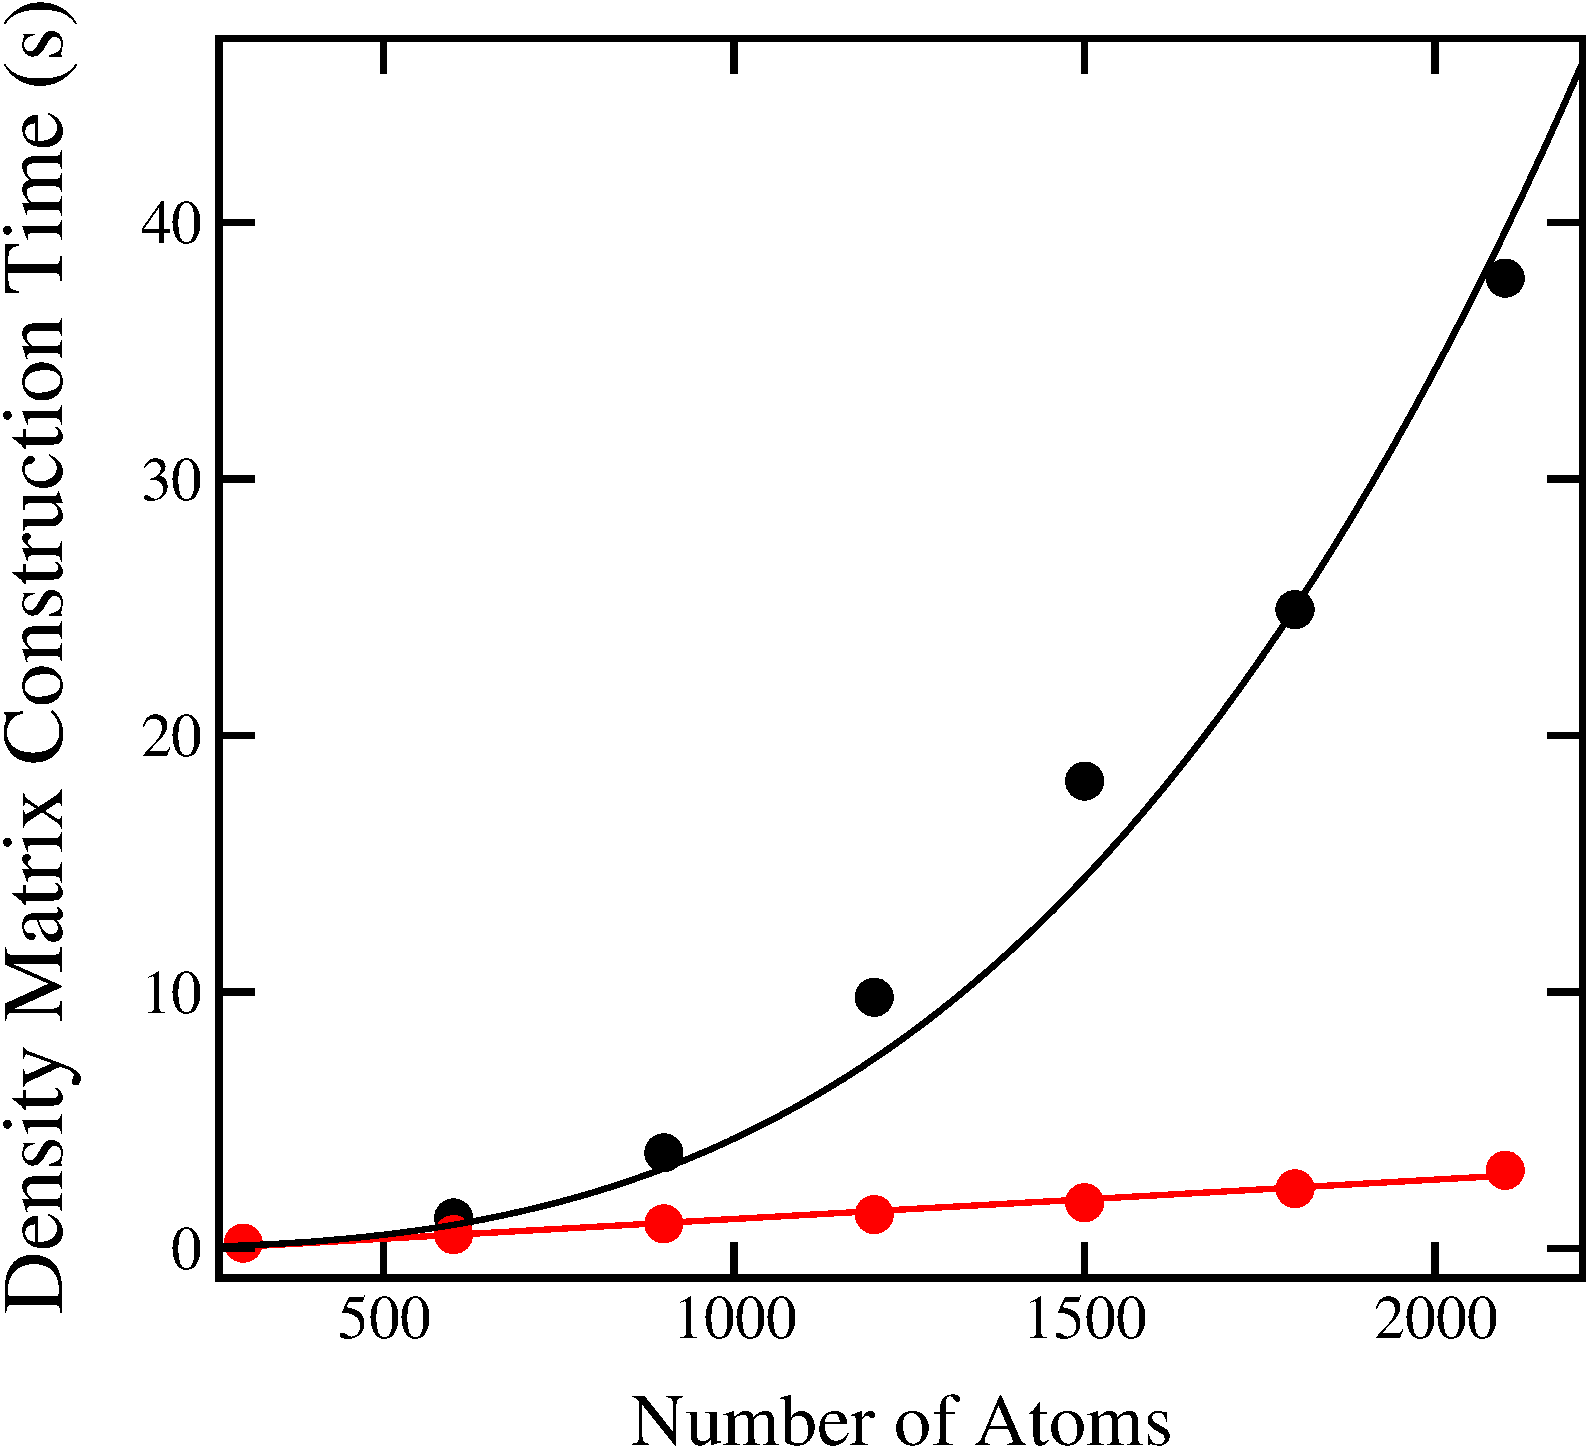
\includegraphics[width=7.0cm]{./fig/times.pdf}
    \caption{SP2 execution times showing performance differences between the dense and ELLPACK-R matrix formats.}
    \label{ellvsdense}
    \end{center}
  \end{figure} 

%
Figure \ref{ellvsdense} shows linear scaling for the ELLPACK-R SP2 method. In comparison, the dense-base SP2 method scales as $\mathcal{O}(N^3)$. The ELLPACK-R matrix-matrix multiply is implemented as in \cite{Mniszewski2015}, while for dense, a BLAS Level 3 DGEMM call is made.

We have shown how a linear algebra based quantum chemistry solver such as the SP2 algorithm can be easily coded up in a high-level style where matrix formats and matrix operations are performed at the library level. Switching from one matrix format to the other can be done at execution time and the performance of the whole code can be easily tested. 

We have introduced the BML library to perform different matrix operations where the format can be decided at runtime. We are continuously extending the supported formats and adding more functionality. The freedom of choosing any matrix format type allows a user to concentrate on the development of high level solvers code quickly. This library has been developed for ease of use in writing quantum chemistry programs.


% \section*{References}
% \bibliographystyle{elsarticle-num} 
% \bibliography{article}

 
